\section{Le maillage}

On a utilisé 2 maillages pour mener les experiences numériques : un maillage
pour le four vide, et un autre maillage avec un aliment sphérique
dans le four (une boulette, peut-être).

Les 2 maillages ont été créés avec le script FreeFEM,
\verb|generate_oven_mesh_3d.edp|.

\begin{figure}[H]
    \centering
    \begin{subfigure}{.5\textwidth}
        \centering
        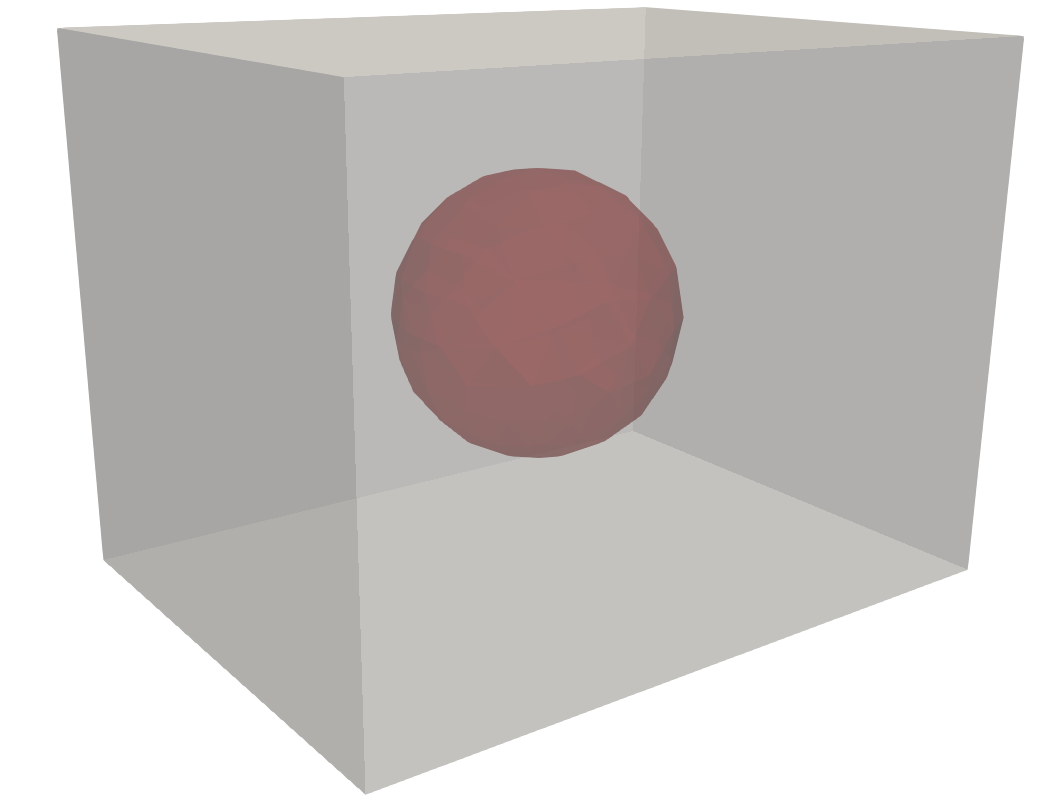
\includegraphics[scale=0.20]{figures/maillage/maillage1.png}
    \end{subfigure}%
    \begin{subfigure}{.5\textwidth}
        \centering
        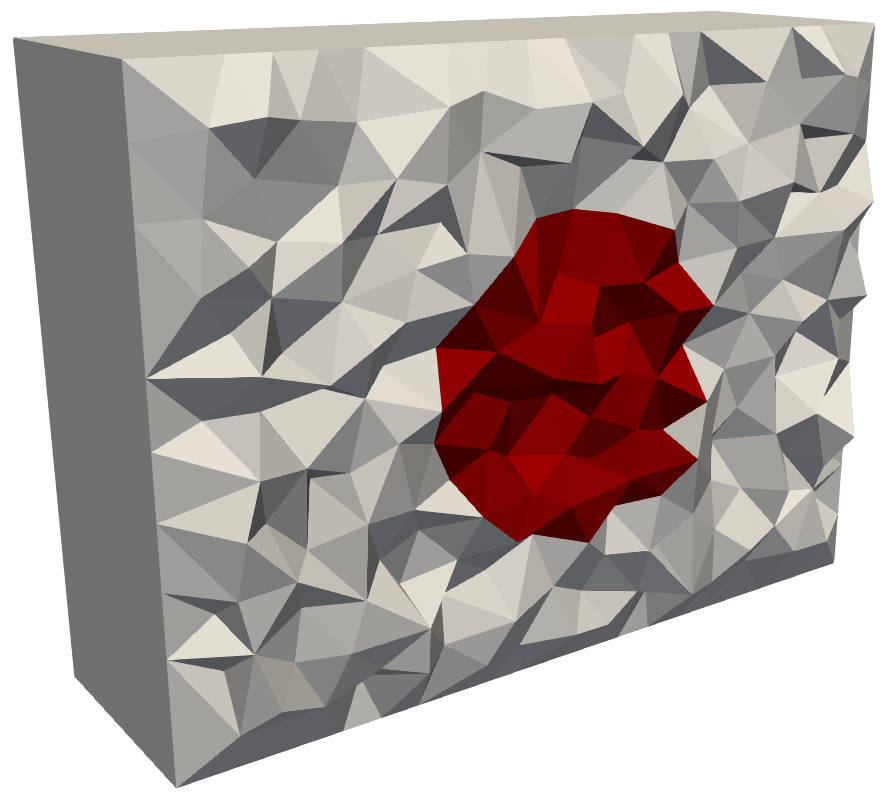
\includegraphics[scale=0.20]{figures/maillage/maillage2.png}
    \end{subfigure}
    \caption{Le maillage du four avec l'aliment dedans.}
\end{figure}
